% Mobile ad-hoc network
% Author: Dr. Ludger Humbert
% Source: https://haspe.homeip.net/projekte/ddi/browser/tex/pgf2
\documentclass{standalone}

\usepackage{tikz}
\usepackage{pgf}

\usepackage{xxcolor}

\usetikzlibrary{arrows,shadows,petri}
%                              wg. tokens
\newlength{\imagewidth}
\newlength{\imagescale}

\listfiles

\begin{document}

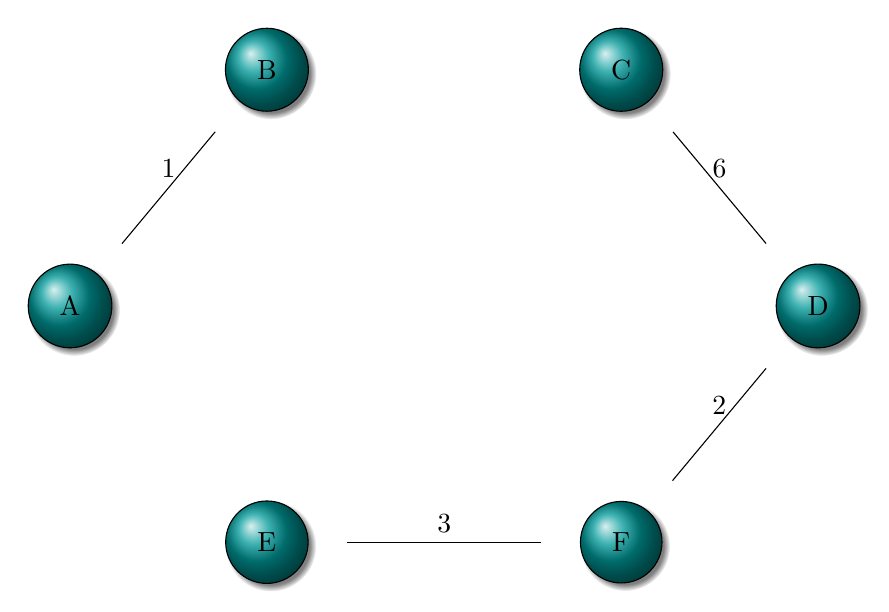
\begin{tikzpicture}[
    knoten/.style={
      shading=ball,
      circle,
      inner sep=.25cm,
      outer sep=.5cm,
      circular drop shadow,
      draw},
    /schriftstueck/.code 2 args={
      \fill[red!50, opacity=#2] #1 rectangle +(.6,.7);
      \foreach \y in {0pt,2pt,4pt,6pt,8pt,10pt,12pt,14pt}
       \draw [yshift=\y, opacity=#2] #1+(0.1,0.1) -- +(0.1,0.1);
      }
    ]

  \node at (2,-2.5) (knoten0) [knoten, ball color=cyan!60!black] {A};
  \node at (4.5,.5) (knoten1) [knoten, ball color=cyan!60!black] {B};
  \node at (9,.5) (knoten2) [knoten, ball color=cyan!60!black] {C};
  \node at (11.5,-2.5) (knoten3) [knoten, ball color=cyan!60!black] {D};
  


  \node at (4.5,-5.5) (knoten4) [knoten, ball color=cyan!60!black] {E};
  \node at (9,-5.5) (knoten5) [knoten, ball color=cyan!60!black] {F};



  \path[every node/.style={anchor=south,auto=false}]

        (knoten0) edge  node[] {$1$} (knoten1)

        (knoten2) edge  node[] {$6$} (knoten3)
        (knoten3) edge  node[] {$2$} (knoten5)
        (knoten5) edge  node[] {$3$} (knoten4)


   ;



\end{tikzpicture}

\end{document}
